


\documentclass{article}
\usepackage{helvet}
\usepackage{cite}
\usepackage{amsmath,amssymb,amsfonts}
\usepackage{algorithmic}
\usepackage{graphicx}
\usepackage{textcomp}
\usepackage{xcolor}
\usepackage{hyperref}
\usepackage{placeins}
\usepackage{subcaption}
\usepackage{physics}
\usepackage{float}

\title{Question 3: Assignment 3: CS 663, Fall 2024}
\author{
    \IEEEauthorblockN{
        \begin{tabular}{cccc}
            \begin{minipage}[t]{0.23\textwidth}
                \centering
                Amitesh Shekhar\\
                IIT Bombay\\
                22b0014@iitb.ac.in
            \end{minipage} & 
            \begin{minipage}[t]{0.23\textwidth}
                \centering
                Anupam Rawat\\
                IIT Bombay\\
                22b3982@iitb.ac.in
            \end{minipage} & 
            \begin{minipage}[t]{0.23\textwidth}
                \centering
                Toshan Achintya Golla\\
                IIT Bombay\\
                22b2234@iitb.ac.in
            \end{minipage} \\
        \end{tabular}
    }
}

\date{September 24, 2024}

\usepackage[margin=0.5in]{geometry}

\begin{document}
\maketitle

\begin{enumerate}
    \item Consider the two images in the homework folder ‘barbara256.png’ and ‘kodak24.png’. Add zero-mean Gaussian noise with standard deviation $\sigma = 5$ to both of them. Implement a mean shift-based filter and show the outputs of the mean shift filter on both images for the following parameter configurations:
    \\

    \begin{figure}[H]
        \centering
        \begin{minipage}{0.48\textwidth}
            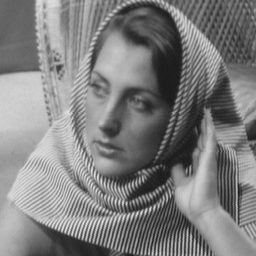
\includegraphics[width=\linewidth]{hw3/q3/barbara256.png}
        \end{minipage}
        \hfill
        \begin{minipage}{0.48\textwidth}
            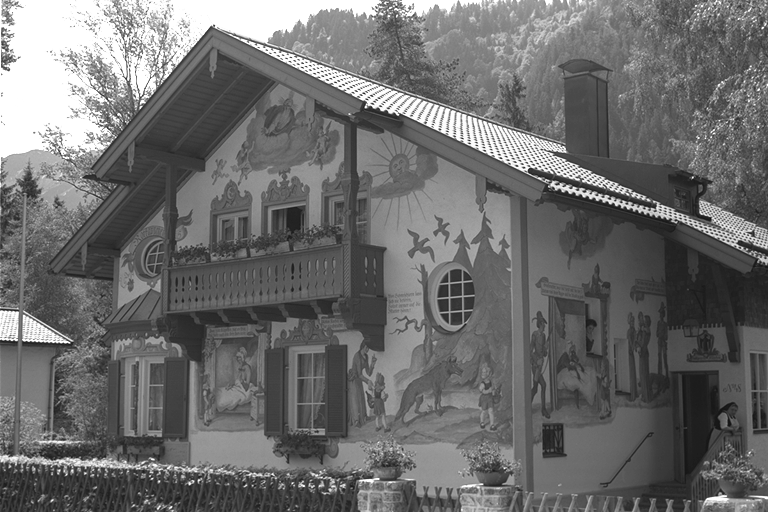
\includegraphics[width=\linewidth]{hw3/q3/kodak24.png}
        \end{minipage}
        \caption{Comparison of barbara256 (left) and kodak24 (right) original images}
    \end{figure}
    
    \subsection{$\sigma_{noise}=5$}
    \begin{figure}[H]
        \centering
        \begin{minipage}{0.48\textwidth}
            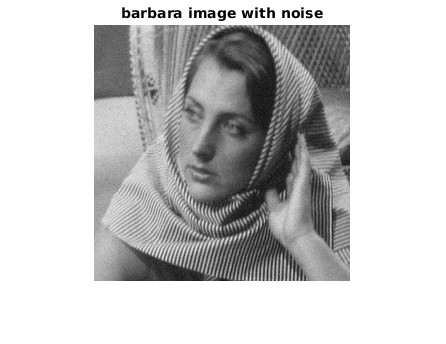
\includegraphics[width=\linewidth]{hw3/q3/barbara_noisy_n5.jpg}
        \end{minipage}
        \hfill
        \begin{minipage}{0.48\textwidth}
            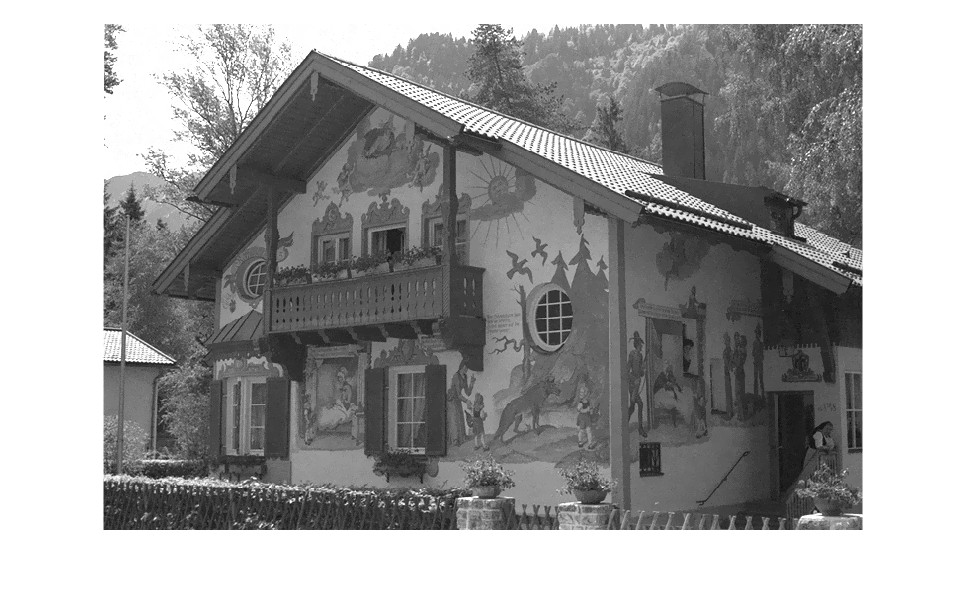
\includegraphics[width=\linewidth]{hw3/q3/kodak_noisy_n5.jpg}
        \end{minipage}
        \caption{Comparison of barbara256 (left) and kodak24 (right) with noise ($\sigma_{noise}=5$)}
    \end{figure}

     \item $\sigma_{s}=2$ and $\sigma_{r}=2$
        \begin{figure}[H]
        \centering
        \begin{minipage}{0.48\textwidth}
            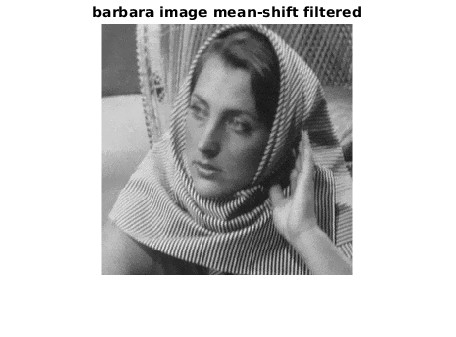
\includegraphics[width=\linewidth]{hw3/q3/barbara_filtered_n5_s2_r2.jpg}
        \end{minipage}
        \hfill
        \begin{minipage}{0.48\textwidth}
            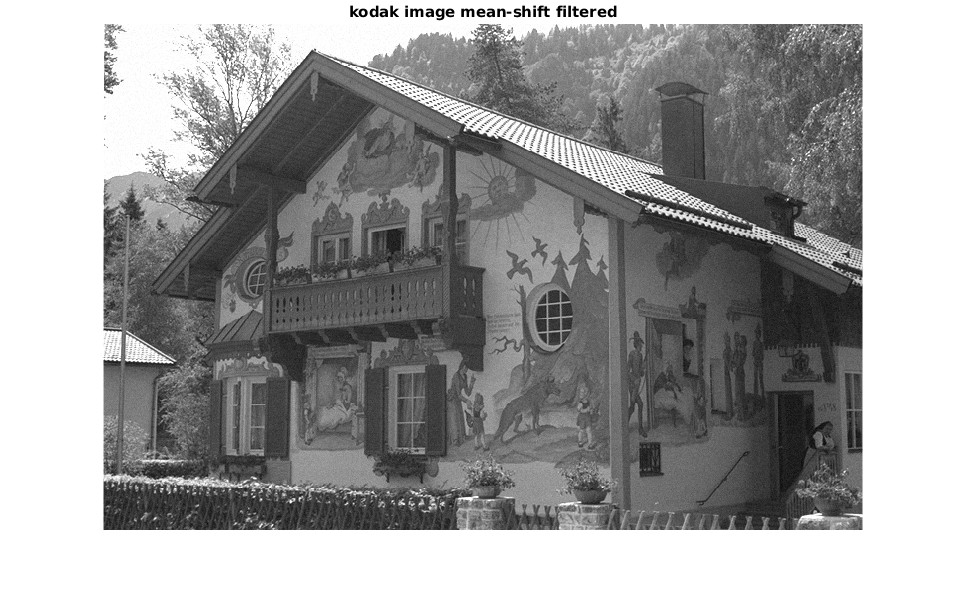
\includegraphics[width=\linewidth]{hw3/q3/kodak_filtered_n5_s2_r2.jpg}
        \end{minipage}
        \caption{Comparison of barbara256 (left) and kodak24 (right) images after mean shift filtering ($\sigma_{s}=2$, $\sigma_{r}=2$)}
    \end{figure}
\newpage
    
    \item $\sigma_{s}=3$ and $\sigma_{r}=15$
    
    \begin{figure}[H]
        \centering
        \begin{minipage}{0.5\textwidth}
            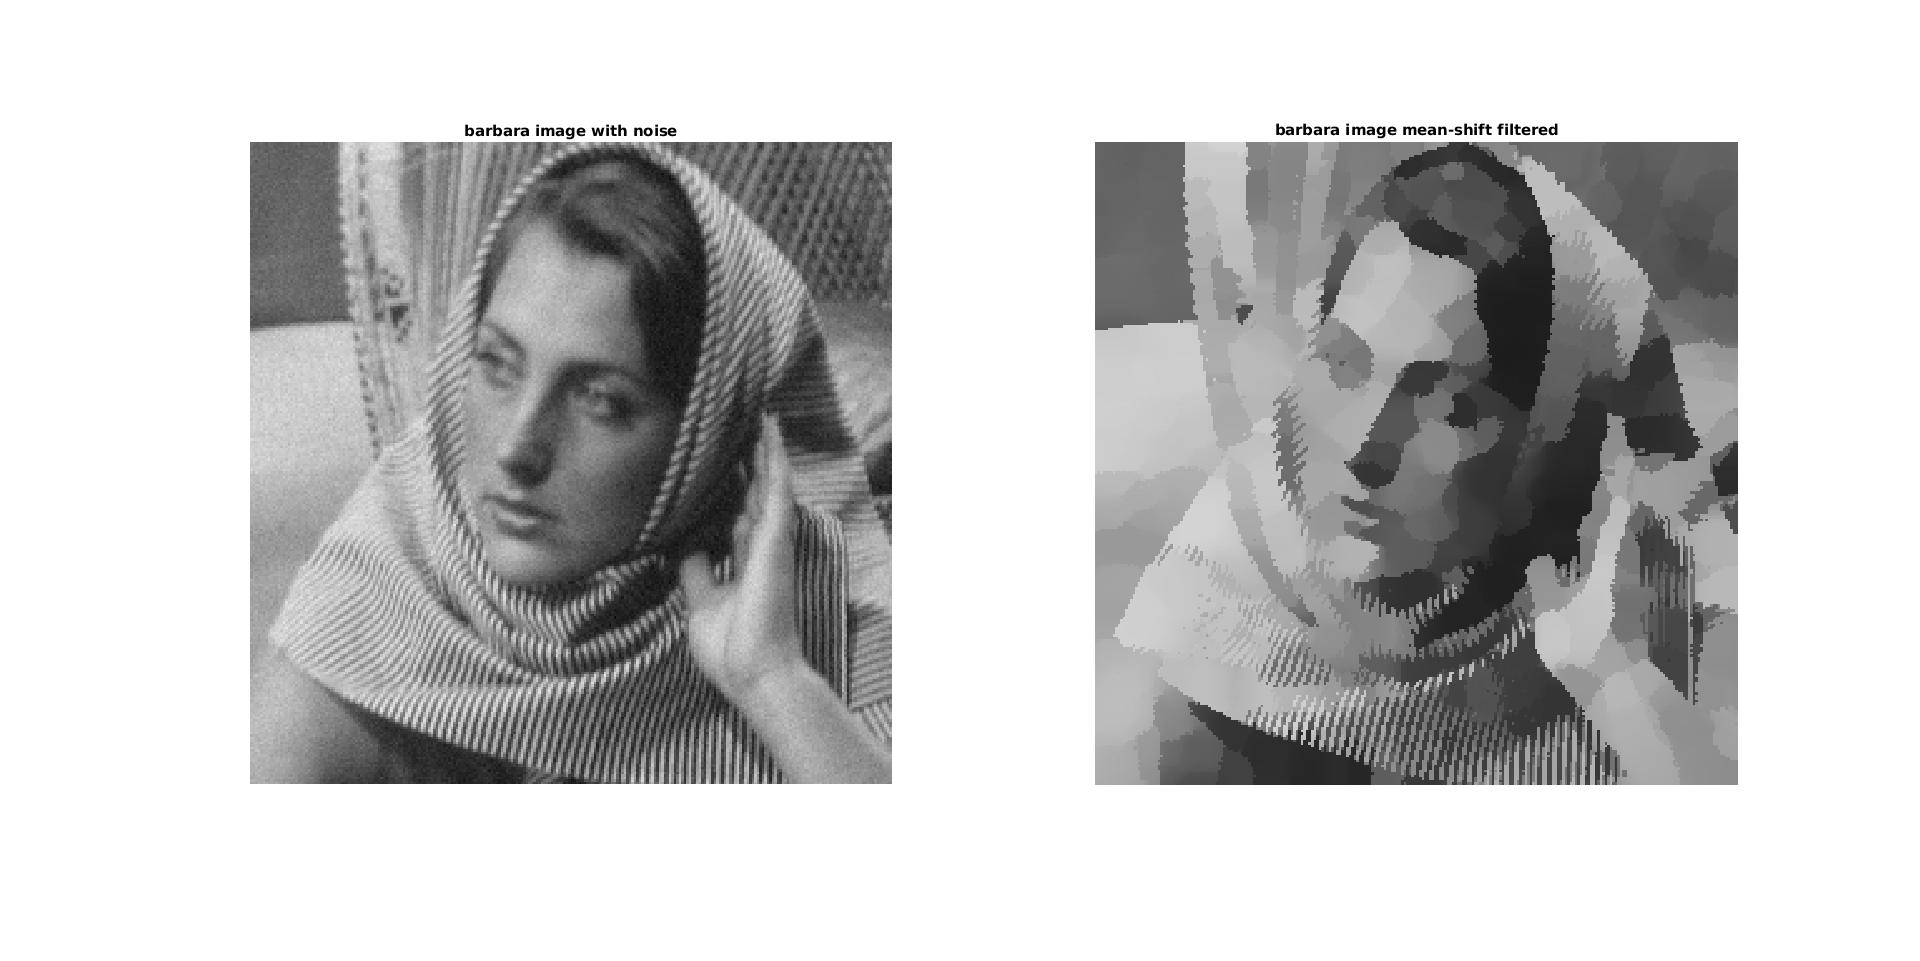
\includegraphics[width=\linewidth]{hw3/q3/sigma_n_5_sigma_s_3_sigma_r_15_barbara.jpg}
        \end{minipage}
        \hfill
        \begin{minipage}{0.5\textwidth}
            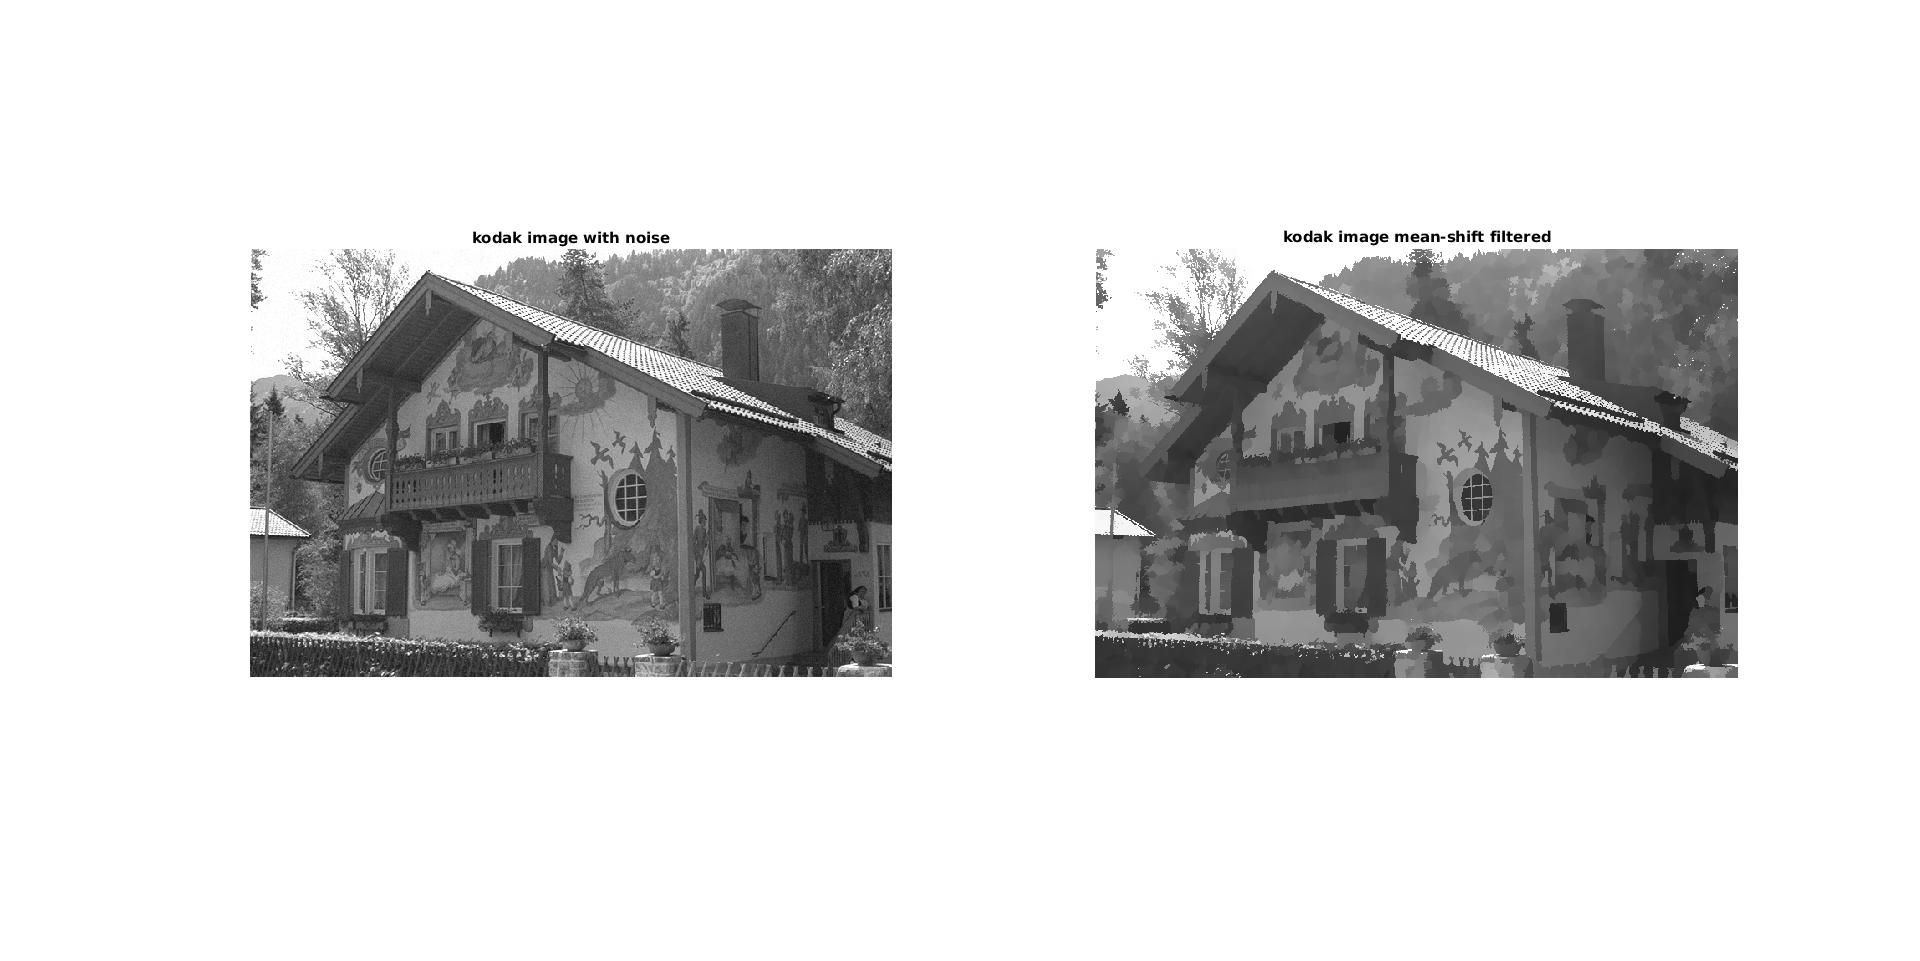
\includegraphics[width=\linewidth]{hw3/q3/sigma_n_5_sigma_s_3_sigma_r_15_kodak.jpg}
        \end{minipage}
        \caption{Comparison of barbara256 (left) and kodak24 (right) images after mean shift filtering ($\sigma_{s}=3$, $\sigma_{r}=15$)}
    \end{figure}

    \item $\sigma_{s}=15$ and $\sigma_{r}=3$
    
    \begin{figure}[H]
        \centering
        \begin{minipage}{0.48\textwidth}
            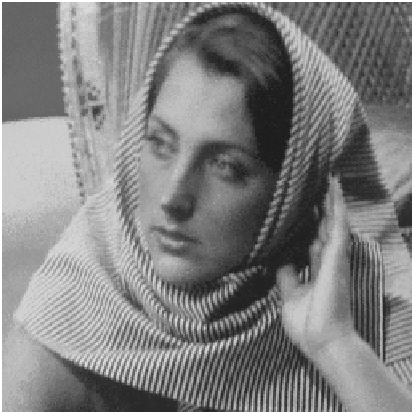
\includegraphics[width=\linewidth]{hw3/q3/barbara_n5_s15_r3.jpg}
        \end{minipage}
        \hfill
        \begin{minipage}{0.48\textwidth}
            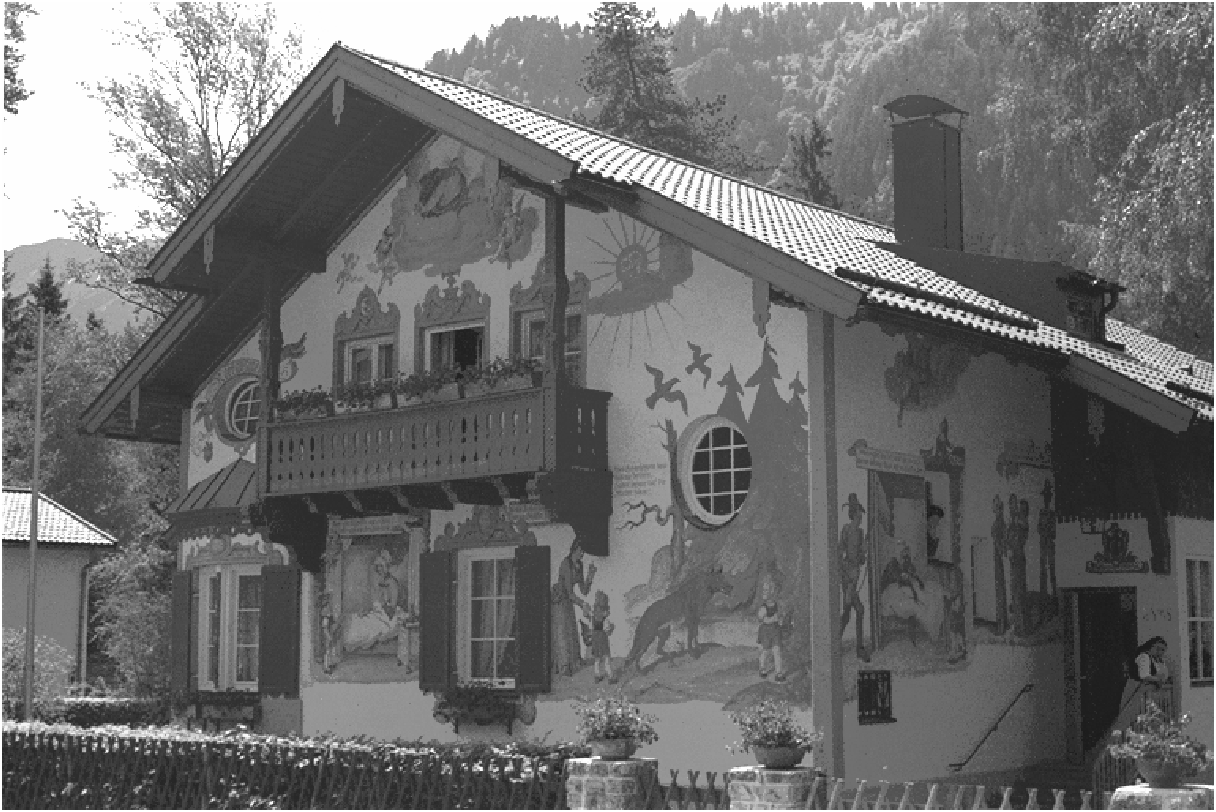
\includegraphics[width=\linewidth]{hw3/q3/kodak_n5_s15_r3.jpg}
        \end{minipage}
        \caption{Comparison of barbara256 (left) and kodak24 (right) images after mean shift filtering ($\sigma_{s}=15$, $\sigma_{r}=3$)}
    \end{figure}
%%%%%%%%%%%%%%%%%%%%%%%%%%%%%%%
%%%%%%%%%%%%%%%%%%%%%%%%%%%%%%
%%%%%%%%%%%%%%%%%%%%%%%%%%%%%
\subsection{$\sigma_{noise}=10$}
    \begin{figure}[H]
        \centering
        \begin{minipage}{0.48\textwidth}
            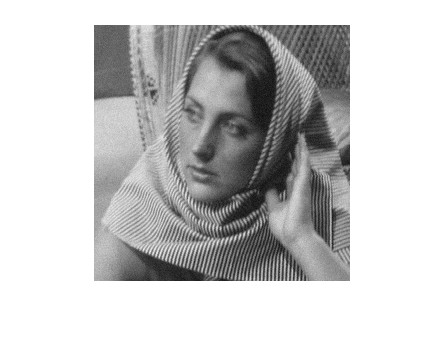
\includegraphics[width=\linewidth]{hw3/q3/barbara_n10_noisy.jpg}
        \end{minipage}
        \hfill
        \begin{minipage}{0.48\textwidth}
            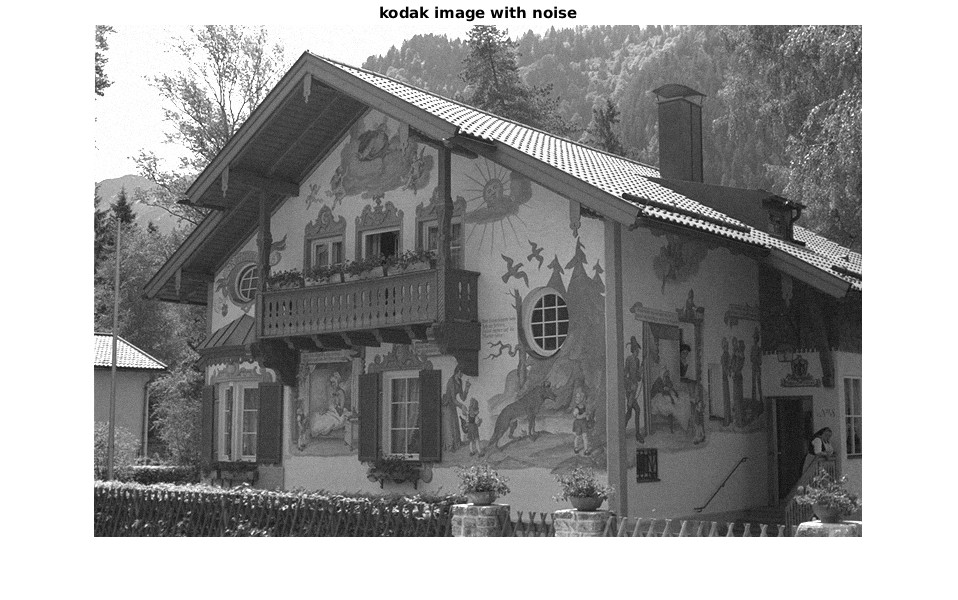
\includegraphics[width=\linewidth]{hw3/q3/kodak_n10_noisy.jpg}
        \end{minipage}
        \caption{Comparison of barbara256 (left) and kodak24 (right) with noise ($\sigma_{noise}=5$)}
    \end{figure}

     \item $\sigma_{s}=2$ and $\sigma_{r}=2$
        \begin{figure}[H]
        \centering
        \begin{minipage}{0.5\textwidth}
            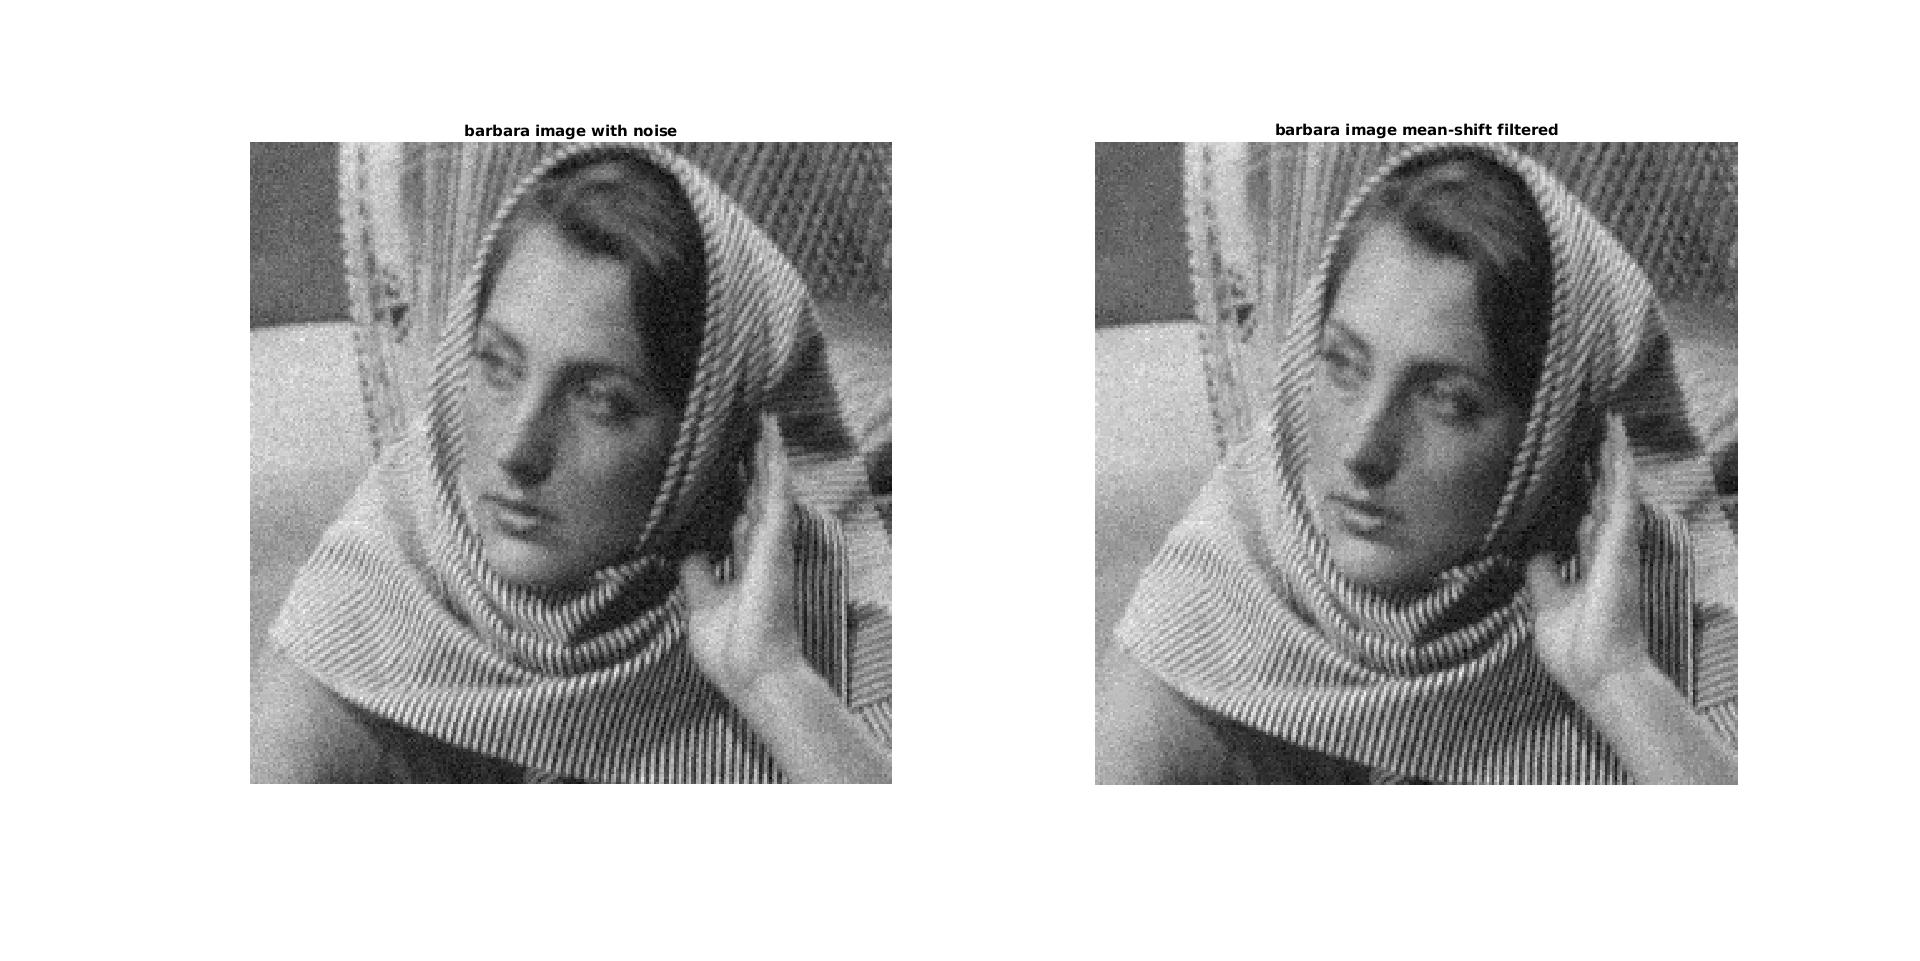
\includegraphics[width=\linewidth]{hw3/q3/sigma_n_10_sigma_s_2_sigma_r_2_barbara.jpg}
        \end{minipage}
        \hfill
        \begin{minipage}{0.5\textwidth}
            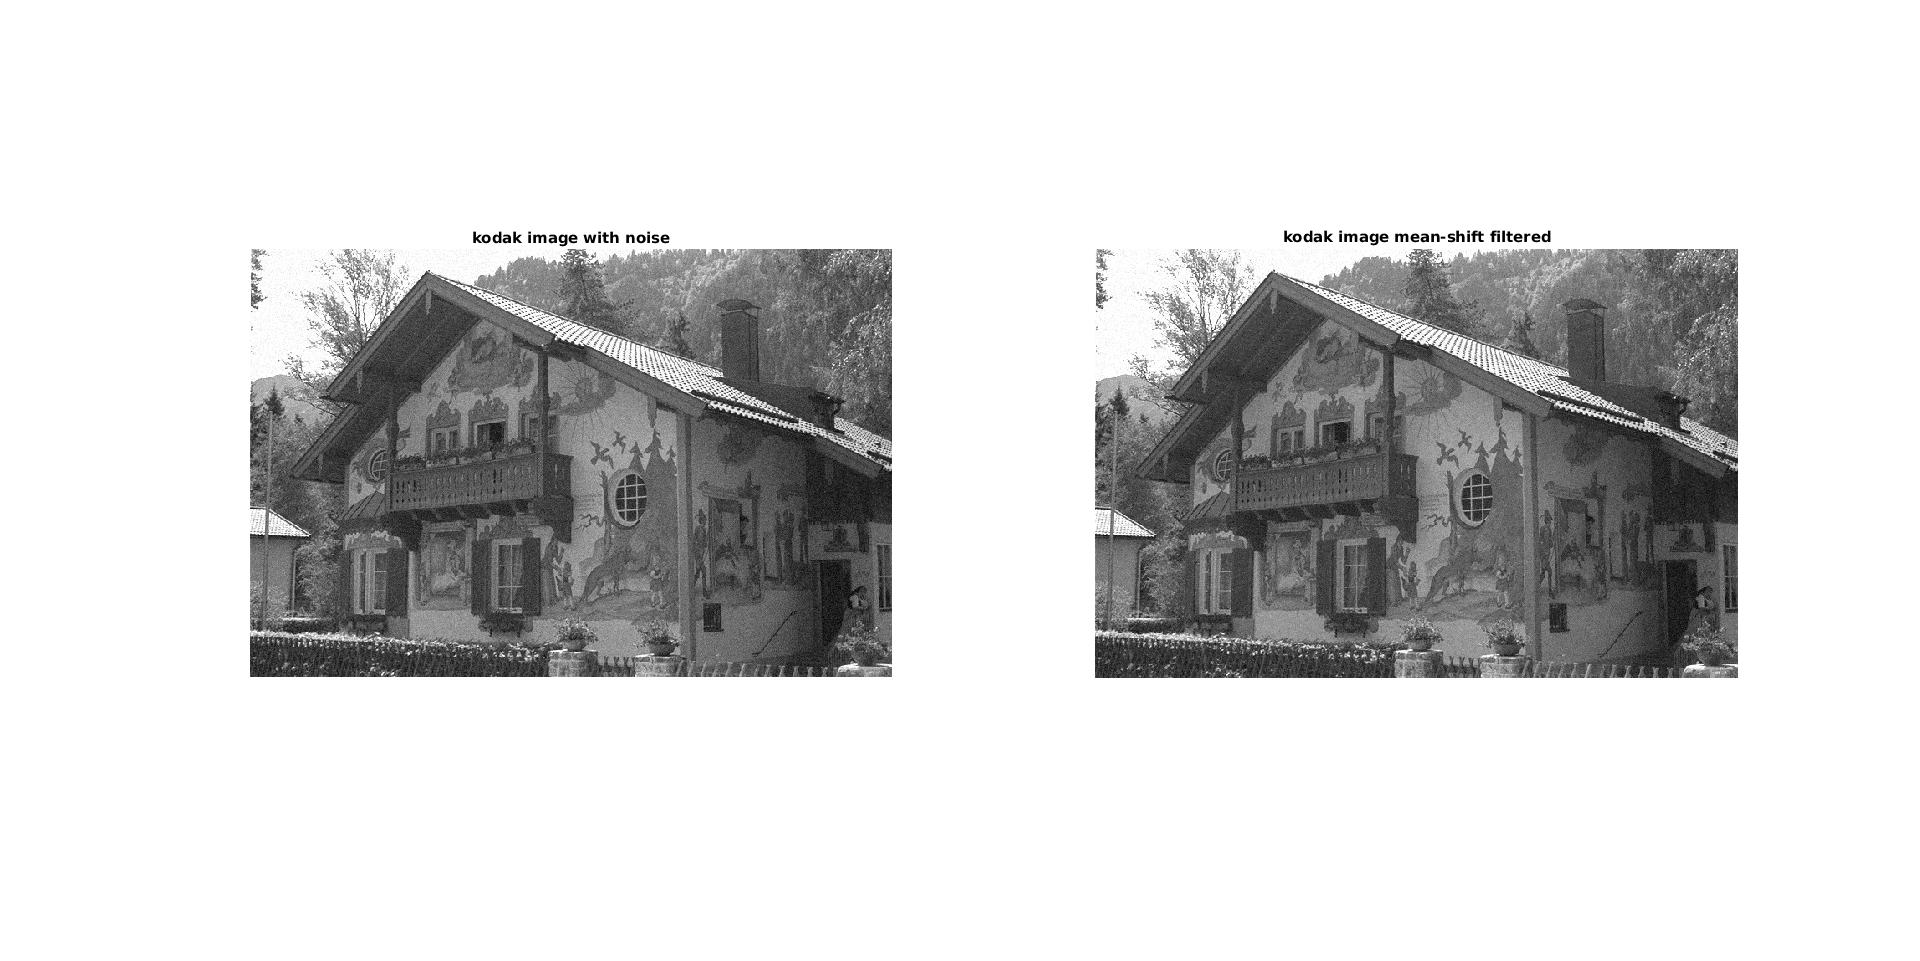
\includegraphics[width=\linewidth]{hw3/q3/sigma_n_10_sigma_s_2_sigma_r_2_kodak.jpg}
        \end{minipage}
        \caption{Comparison of barbara256 (left) and kodak24 (right) images after mean shift filtering ($\sigma_{s}=2$, $\sigma_{r}=2$)}
    \end{figure}
\newpage
    
    \item $\sigma_{s}=3$ and $\sigma_{r}=15$
    
    \begin{figure}[H]
        \centering
        \begin{minipage}{0.48\textwidth}
            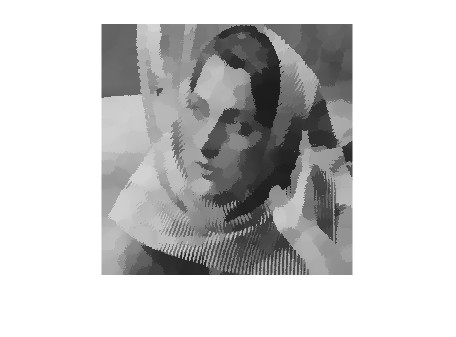
\includegraphics[width=\linewidth]{hw3/q3/barbara_n10_s3_r15.jpg}
        \end{minipage}
        \hfill
        \begin{minipage}{0.48\textwidth}
            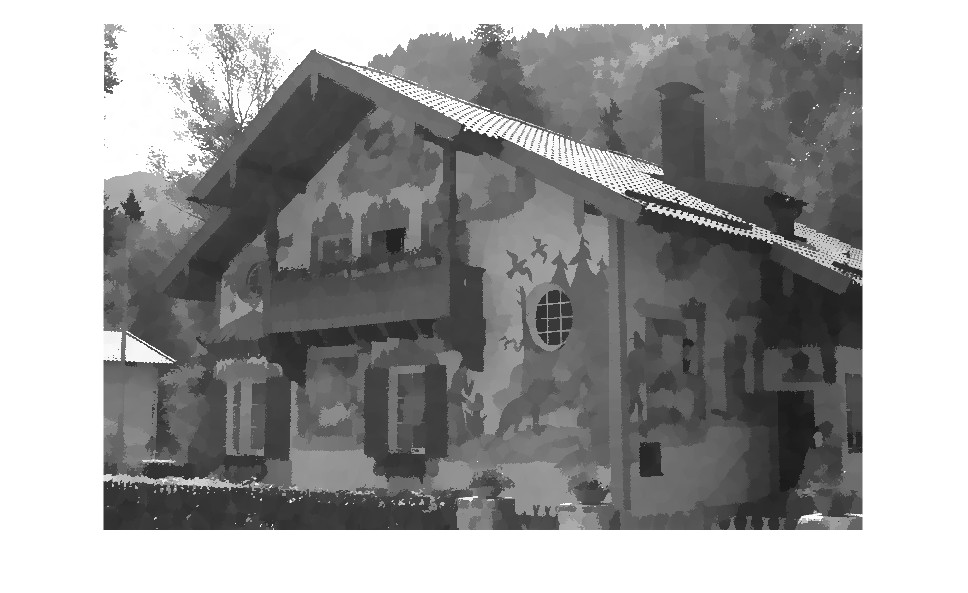
\includegraphics[width=\linewidth]{hw3/q3/kodak_n10_s3_r15.jpg}
        \end{minipage}
        \caption{Comparison of barbara256 (left) and kodak24 (right) images after mean shift filtering ($\sigma_{s}=3$, $\sigma_{r}=15$)}
    \end{figure}

    \item $\sigma_{s}=15$ and $\sigma_{r}=3$
    
    \begin{figure}[H]
        \centering
        \begin{minipage}{0.48\textwidth}
            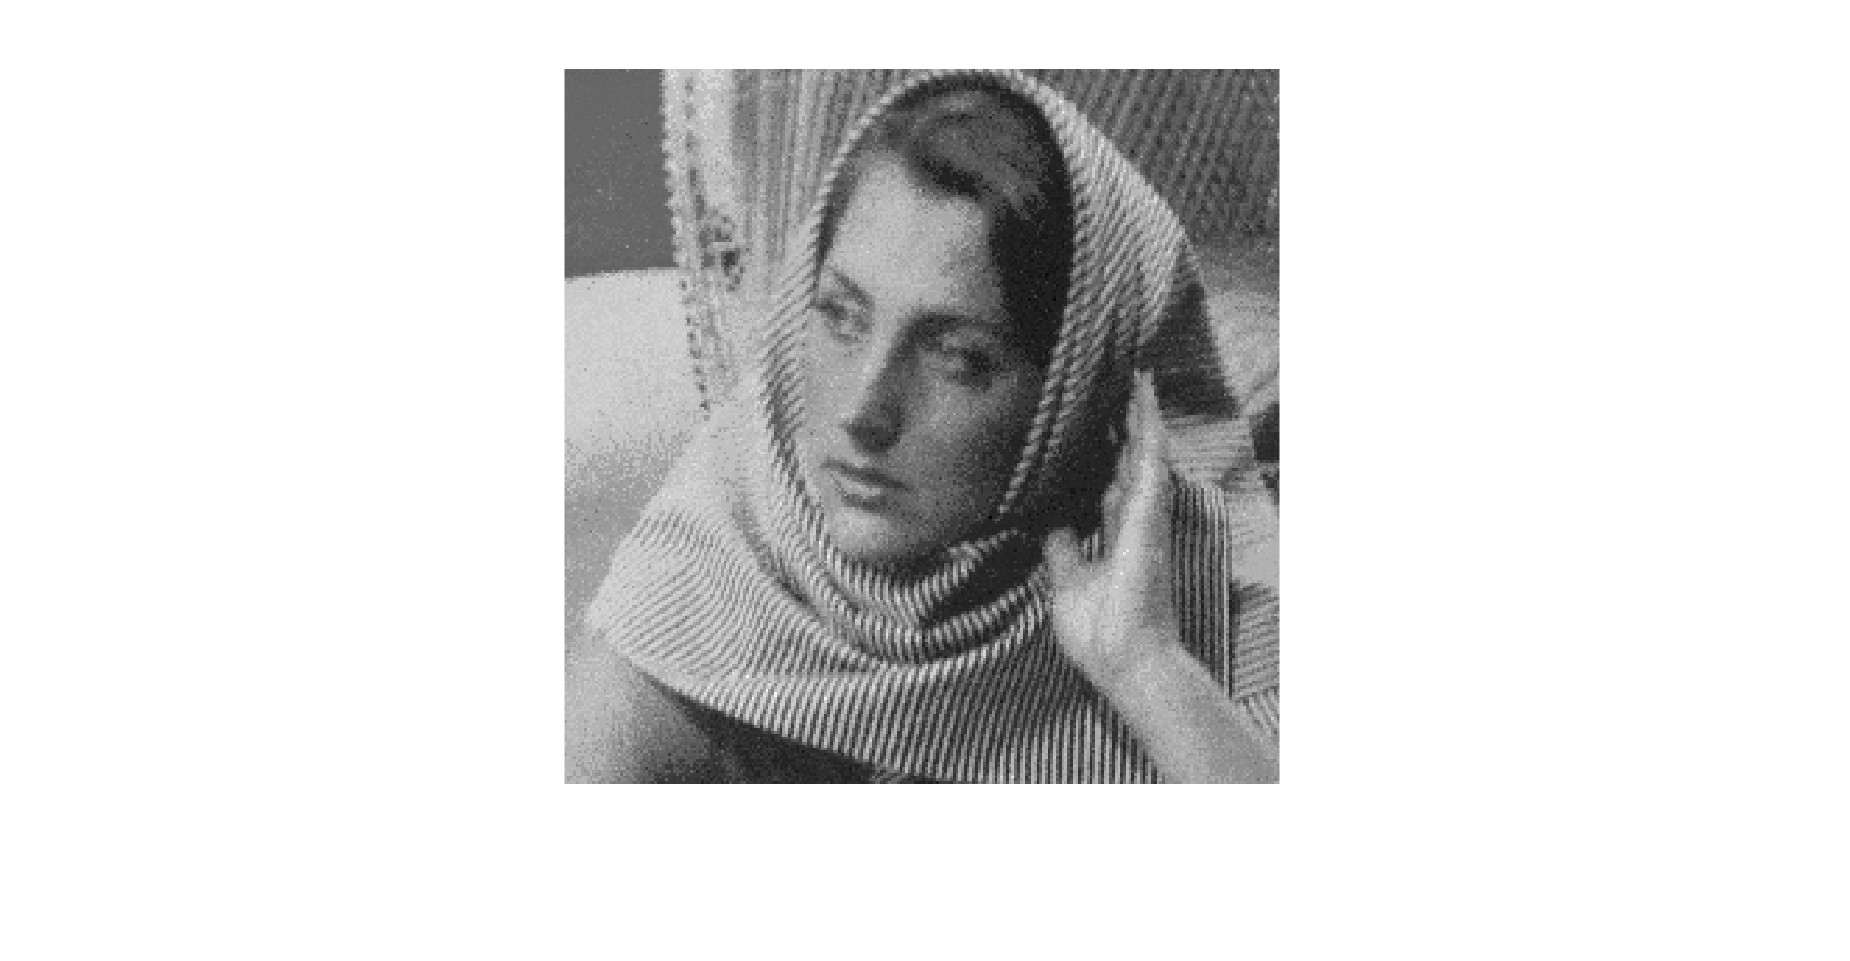
\includegraphics[width=\linewidth]{hw3/q3/barbara_n10_s15_r3.jpg}
        \end{minipage}
        \hfill
        \begin{minipage}{0.48\textwidth}
            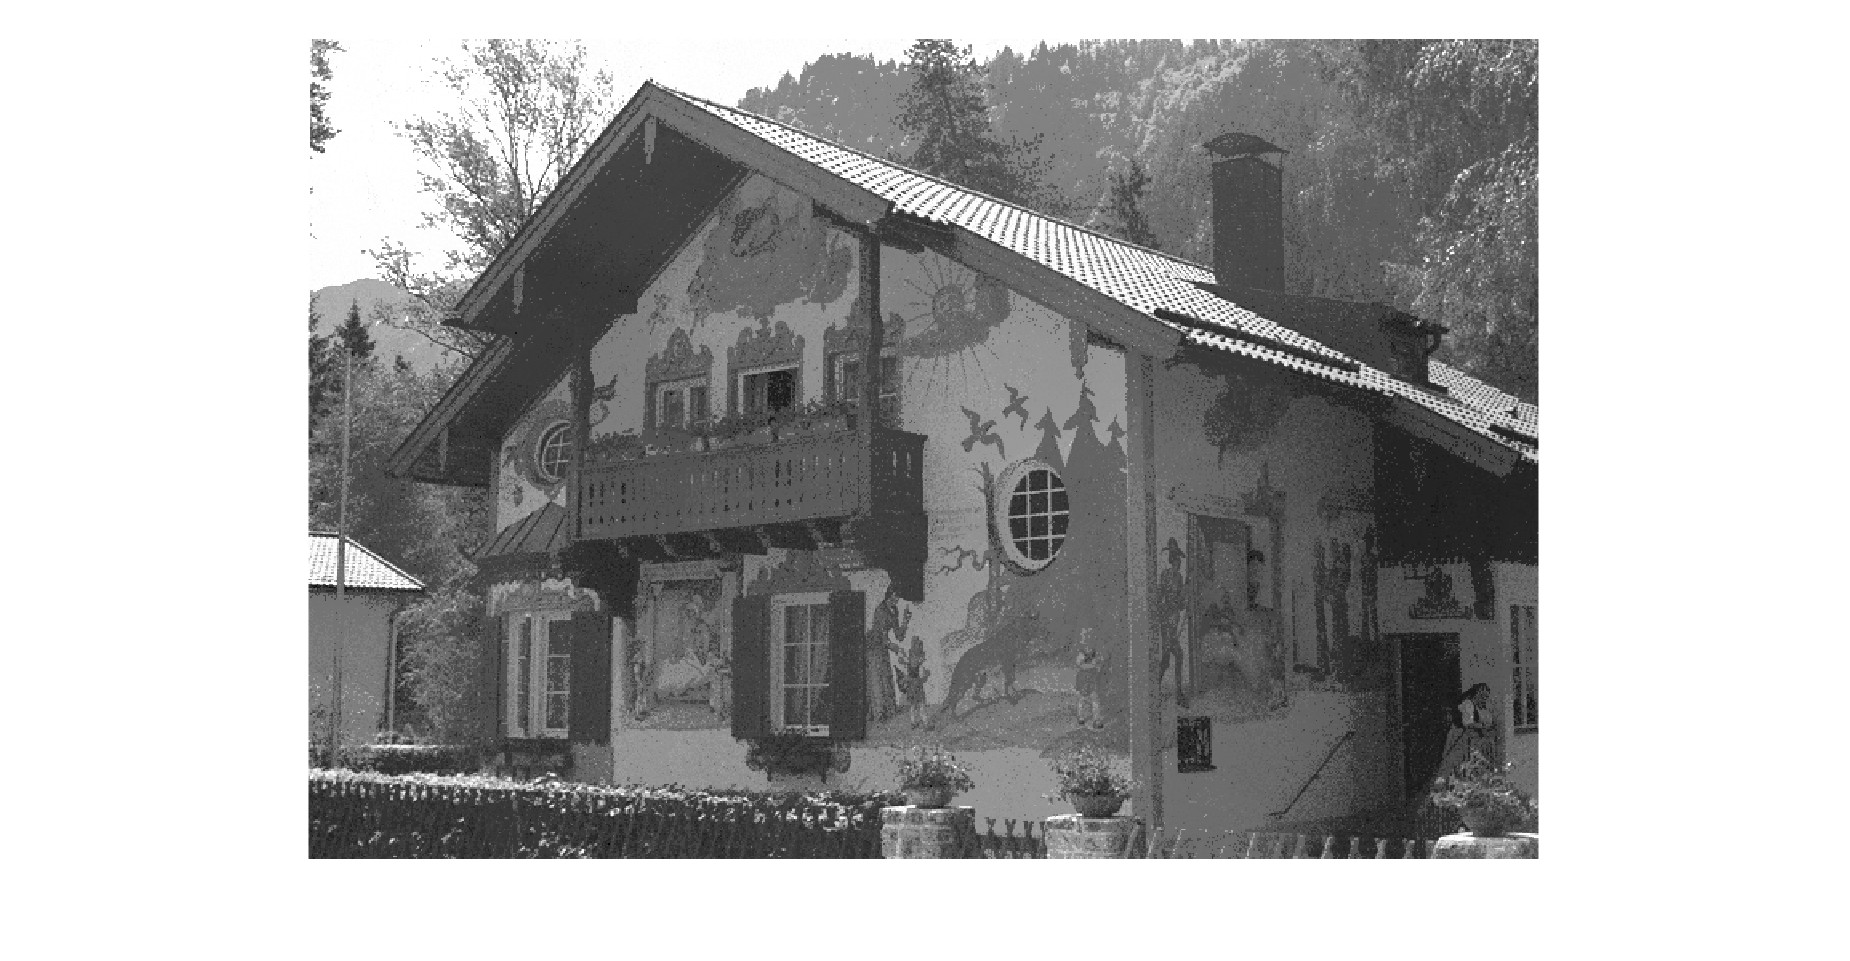
\includegraphics[width=\linewidth]{hw3/q3/kodak_n10_s15_r3.jpg}
        \end{minipage}
        \caption{Comparison of barbara256 (left) and kodak24 (right) images after mean shift filtering ($\sigma_{s}=15$, $\sigma_{r}=3$)}
    \end{figure}

\end{enumerate}

\subsection{Comments}
The threshold $\epsilon$ is set as 0l.01. Even at this threshold, the computation time for large $\sigma_{s}$ and $\sigma_{r}$ were becoming very large ($>$>20min), hence we didn't reduce it further.
In first case, when gaussian noise of standard deviation = 5 is added, we  see that as $\sigma _{s}$ (spatial parameter) and $\sigma_{r}$ (intensity bandwith) increases, the neighbourhood size across which local maxima computation is done. This in turn makes the filtering more aggressive. This happens because as$\sigma _{s}$ or $\sigma _{r}$ increases, there are fewer local-maximas in each window.\\
As we increase $\sigma_{s}$(large spatial bandwidth), the filter will consider a larger spatial neighborhood, meaning it will smooth over a broader area. Pixels that are far apart (spatially) will still influence each other.\\
Similarly, When we increase$\sigma_{r}$,: The filter will allow pixels with larger intensity differences to influence each other. The filter will smooth more across different intensity levels, resulting in less edge preservation (similar to bilateral filtering).
As $\sigma$ of the Gaussian noise increases, the convergence time has reduced. Also,the effects of filtering is more pronounced. \\
The convergence time for $\sigma_{s}=15$ case was too long and our system crashed a couple of times in doing so. Hence we have not included those in our report.
\end{document}

